\documentclass[conference]{IEEEtran}
\IEEEoverridecommandlockouts

\usepackage{cite}
\usepackage{amsmath,amssymb,amsfonts}
\usepackage{algorithmic}
\usepackage{graphicx}
\usepackage{textcomp}
\usepackage{xcolor}
\usepackage{float}
\usepackage{booktabs}
\usepackage{tikz}
\usetikzlibrary{shapes,arrows,positioning,calc,shadows,shapes.geometric}

\def\BibTeX{{\rm B\kern-.05em{\sc i\kern-.025em b}\kern-.08em
    T\kern-.1667em\lower.7ex\hbox{E}\kern-.125emX}}
\begin{document}

\title{DS-PAH-GNN: Deep Structured Physics-Aware Hierarchical Graph Neural Network for Real-Time Topology Optimisation in DC Microgrids
}

\author{
\IEEEauthorblockN{
\begin{tabular}{@{}p{0.45\textwidth}@{\hspace{0.05\textwidth}}p{0.45\textwidth}@{}}
\begin{center}
Aditi Ramakrishnan\\
\textit{Department of Electrical and Electronics Engineering}\\
\textit{Christ (Deemed to be University)}\\
Bengaluru, Karnataka\\
aditirkrishna@gmail.com
\end{center}
&
\begin{center}
Manisha Kumari Joshi\\
\textit{Department of Electrical and Electronics Engineering}\\
\textit{Christ (Deemed to be University)}\\
Bengaluru, India\\
manishakumarijoshi12@gmail.com
\end{center}
\\[1.2em]
\begin{center}
Srusti M. Suryavanshi\\
\textit{Department of Electrical and Electronics Engineering}\\
\textit{Christ (Deemed to be University)}\\
Bengaluru, India\\
srustisuryavanshi@gmail.com
\end{center}
&
\begin{center}
Dr. Vijaya Margaret\\
\textit{Department of Electrical and Electronics Engineering}\\
\textit{Christ (Deemed to be University)}\\
Bengaluru, India\\
\subsection{Baselines and Comparative Models}

To quantify the benefit of explicitly embedding electrical physics into the learning architecture, we evaluate two simple baselines alongside DS-PAH-GNN:
\begin{enumerate}
    \item \textbf{Vanilla Heterogeneous GNN}: a model with the same heterogeneous node partitioning and message-passing topology but which omits physics-aware edge encodings (edge attributes set to constant values). This baseline isolates the contribution of conductance-informed messages.
    \item \textbf{Small MLP on Hand-Crafted Features}: a lightweight multilayer perceptron trained on aggregated features such as total system load, mean line conductance, and the number of closed tie-lines. This baseline evaluates the value of structural graph representations versus simple summary statistics.
\end{enumerate}

Each baseline is trained using an identical protocol (optimizer, scheduler, and data splits) so that comparisons reflect model inductive biases rather than training recipe differences.

\subsection{Generalization Test: Unseen Topologies}

We design a focused generalization experiment to confirm that the model learns physics-informed mappings rather than memorizing specific graphs. The protocol is:
\begin{itemize}
    \item Partition the dataset by topology family: \emph{training} snapshots contain only radial configurations (all tie-lines open), while \emph{test} snapshots contain at least one closed tie-line (non-radial configurations).
    \item Train models solely on the radial subset and evaluate on the non-radial hold-out. Report $R^2$, MAE and RMSE to quantify generalization gap.
    \item Repeat across several random seeds and topology samplings to ensure robustness of the conclusions.
\end{itemize}

This experiment provides a stringent check: if the GNN retains strong predictive accuracy on topologies that were never seen during training, we can be confident the model has learned physics-consistent behavior rather than dataset-specific patterns.

\section{Results and Discussion}
\end{center}
\end{tabular}
}
}


\maketitle

\begin{abstract}
The rapid electrification of transportation demands advanced control strategies for DC microgrids, particularly to accommodate the stochastic and high-power loads introduced by electric vehicle (EV) fast-charging stations. Conventional topology optimization approaches based on iterative numerical solvers are computationally prohibitive for real-time control. In this paper, we present \textbf{DS-PAH-GNN}, a data-driven physics-aware hierarchical graph neural network that serves as a neural surrogate for microgrid physics. The proposed framework introduces a novel heterogeneous graph architecture that explicitly embeds electrical conductance into the message-passing mechanism, thereby mimicking Kirchhoff's laws, and employs Self-Attention Graph Pooling (SAGPool) to dynamically identify critical network components. Trained on a high-fidelity dataset of 600,000 operating snapshots generated using a linearized DC power flow engine, the model achieves an $R^2 > 0.99$ in power-loss prediction. We further demonstrate a real-time topology optimization framework that reduces system losses by more than 60\% during congestion events while operating approximately 100$\times$ faster than traditional solvers. These results bridge the gap between rigorous power system physics and scalable deep learning for next-generation microgrid control.
\end{abstract}

\begin{IEEEkeywords}
DC microgrids, electric vehicle charging, graph neural networks, power flow analysis, topology optimization, hierarchical networks, renewable integration.
\end{IEEEkeywords}

\section{Introduction}

The rapid electrification of transportation is fundamentally reshaping modern power distribution systems. Unlike conventional loads, electric vehicle (EV) charging introduces strong spatiotemporal variability: individual charging stations can demand power in excess of 50~kW, charging events tend to cluster during evening peak hours, and the nonlinear Constant-Current Constant-Voltage (CC--CV) charging behavior of batteries further complicates accurate load modeling. These characteristics collectively challenge the assumptions underlying traditional planning and control tools for distribution networks.

DC microgrids provide a compelling architectural response to these challenges. By eliminating reactive power phenomena, reducing conversion losses by approximately 15--25\%, and enabling direct coupling of photovoltaic generation and battery storage, DC systems offer higher efficiency and simpler control compared to their AC counterparts. However, the reliable operation of EV-centric DC microgrids requires continuous coordination of voltage regulation, thermal constraints, and network losses under highly dynamic operating conditions. Achieving this balance demands computational approaches capable of learning complex nonlinear relationships over heterogeneous and time-varying grid states.

A central operational task in this context is optimal network topology reconfiguration. This problem is naturally formulated as a mixed-integer nonlinear program (MINLP) and is known to be NP-hard. Conventional physics-based solvers, such as Newton--Raphson methods, exhibit cubic computational complexity $\mathcal{O}(N^3)$ with respect to network size, which severely limits their suitability for the sub-second control cycles required for real-time grid stability.

Graph Neural Networks (GNNs) have recently emerged as a promising learning paradigm for power system analysis because they natively represent the topology-dependent structure of electrical networks. In contrast to fully connected neural architectures, GNNs exploit graph connectivity to achieve strong generalization across different network sizes and configurations, making them particularly well-suited for grid modeling and optimization.

In this work, we propose \textbf{DS-PAH-GNN}, a deep structured physics-aware hierarchical graph neural network for real-time topology optimization in DC microgrids. The proposed framework:
\begin{enumerate}
    \item \textbf{Incorporates electrical conductance} $(1/R)$ as edge features to guide message passing, enabling the network to learn a neural surrogate of power flow behavior;
    \item \textbf{Employs Self-Attention Graph Pooling (SAGPool)} to concentrate computational focus on electrically stressed components, such as overloaded stations; and
    \item \textbf{Enables sub-second evaluation} of thousands of candidate network configurations to identify near-optimal topologies suitable for real-time control.
\end{enumerate}


\section{Mathematical Modeling of DC Microgrids}

In this section, we present the mathematical formulation used to model the DC microgrid under study. The objective is to construct a representation that is physically meaningful, computationally efficient, and suitable for optimization and learning-based analysis. To this end, the microgrid is modeled as a hierarchical dual-bus system and expressed using a graph-theoretic abstraction, which allows electrical constraints to be encoded directly into the network topology.

\subsection{Graph Theoretic Formulation}

The DC microgrid is represented as a directed graph
\begin{equation}
\mathcal{G} = (\mathcal{V}, \mathcal{E}),
\end{equation}
where the vertex set $\mathcal{V}$ corresponds to electrical buses and components, and the edge set $\mathcal{E}$ represents the electrical interconnections between them. This abstraction provides a structured framework in which physical properties of the network can be mapped to graph elements.

To reflect the hierarchical organization of the microgrid, the vertex set is partitioned into three disjoint subsets:
\begin{equation}
\mathcal{V} = \mathcal{V}_{root} \cup \mathcal{V}_{station} \cup \mathcal{V}_{device}.
\end{equation}
Here, $\mathcal{V}_{root}$ represents the root node corresponding to the point of common coupling (PCC) with the upstream grid. The set $\mathcal{V}_{station}$ contains intermediate distribution substations that aggregate power flows, while $\mathcal{V}_{device}$ consists of terminal components such as EV chargers, photovoltaic (PV) inverters, and battery energy storage systems (BESS). This partitioning explicitly encodes the functional roles of different nodes within the microgrid.

The edge set $\mathcal{E} \subseteq \mathcal{V} \times \mathcal{V}$ models the DC distribution lines connecting pairs of nodes. Each edge $e_{ij} = (i,j) \in \mathcal{E}$ is associated with a feature vector
\begin{equation}
\mathbf{e}_{ij} = [R_{ij}, S_{ij}]^T,
\end{equation}
where $R_{ij}$ denotes the electrical resistance of the line and $S_{ij} \in \{0,1\}$ indicates the binary switch status. The switch variable captures the reconfigurable nature of the network by allowing lines to be electrically connected or disconnected.

Based on these parameters, the effective electrical conductance of each line is defined as
\begin{equation}
G_{ij} = \frac{S_{ij}}{R_{ij}}.
\end{equation}
This definition ensures that when a switch is open ($S_{ij}=0$), the corresponding conductance becomes zero, effectively removing the line from the network without altering the graph structure.

\begin{figure}[htbp]
\centering
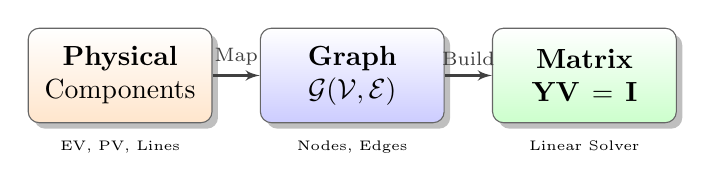
\begin{tikzpicture}[node distance=1.5cm, auto, >=latex']
    \tikzstyle{block} = [rectangle, draw=black!60, fill=blue!5, text width=2.1cm, text centered, rounded corners, minimum height=1.2cm, drop shadow]
    \tikzstyle{line} = [draw, -latex', thick, darkgray]
    
    \node [block, top color=white, bottom color=orange!20] (phys) {\textbf{Physical}\\Components};
    \node [block, top color=white, bottom color=blue!20, right=0.6cm of phys] (graph) {\textbf{Graph}\\$\mathcal{G}(\mathcal{V}, \mathcal{E})$};
    \node [block, top color=white, bottom color=green!20, right=0.6cm of graph] (math) {\textbf{Matrix}\\$\mathbf{Y}\mathbf{V}=\mathbf{I}$};
    
    \draw [line] (phys) -- node[above, font=\scriptsize] {Map} (graph);
    \draw [line] (graph) -- node[above, font=\scriptsize] {Build} (math);
    
    \node [below=0.1cm of phys, font=\tiny, align=center] {EV, PV, Lines};
    \node [below=0.1cm of graph, font=\tiny, align=center] {Nodes, Edges};
    \node [below=0.1cm of math, font=\tiny, align=center] {Linear Solver};
\end{tikzpicture}
\caption{Modeling Abstraction Levels. Physical entities are mapped to graph primitives, which construct the algebraic system solved by the physics engine.}
\label{fig:math_model}
\end{figure}

\subsection{Linearized DC Power Flow}

To enable efficient simulation and facilitate large-scale analysis, a linearized DC power flow model is employed. This model assumes that voltage deviations from the nominal reference voltage $V_{ref}$ are sufficiently small, allowing nonlinear power flow relationships to be approximated linearly.

The electrical state of the system is governed by Kirchhoff's Current Law (KCL) applied at each node, which can be expressed in matrix form as
\begin{equation}
\mathbf{Y}\mathbf{V} = \mathbf{I},
\end{equation}
where $\mathbf{V} \in \mathbb{R}^{N}$ is the vector of nodal voltages, $\mathbf{I} \in \mathbb{R}^{N}$ is the vector of net current injections, and $\mathbf{Y} \in \mathbb{R}^{N \times N}$ is the nodal admittance matrix of the network.

The admittance matrix is constructed using the effective conductances as
\begin{equation}
Y_{ij} =
\begin{cases}
\sum_{k \neq i} G_{ik}, & \text{if } i = j, \\
- G_{ij}, & \text{if } i \neq j,
\end{cases}
\end{equation}
where the diagonal entries represent the total conductance connected to each node, and the off-diagonal entries capture the coupling between adjacent nodes. This structure ensures that the admittance matrix directly reflects the underlying network topology.

Constant-power devices introduce nonlinearities through the relationship between current, power, and voltage. To preserve linearity, the current injection at node $i$ is approximated using the nominal voltage:
\begin{equation}
I_i \approx \frac{P_i^{gen} - P_i^{load}}{V_{ref}}.
\end{equation}
This approximation allows both generation and load to be incorporated into the linear power flow formulation.

The root node is treated as a slack bus with fixed voltage $V_{root} = 1.0$ per unit. Voltages at all remaining nodes are obtained by solving the reduced nodal admittance system, which is computed using LU decomposition for numerical efficiency.

The objective of network reconfiguration is to minimize total Ohmic losses across the microgrid, expressed as
\begin{equation}
P_{loss} = \sum_{(i,j) \in \mathcal{E}} S_{ij} \cdot G_{ij} (V_i - V_j)^2.
\end{equation}
This formulation explicitly links electrical losses to both voltage differences and switch states, thereby coupling system performance with network topology. The optimization is subject to connectivity requirements and nodal voltage constraints
\begin{equation}
V_{min} \leq V_i \leq V_{max}.
\end{equation}

\section{Problem Formulation}

We formalize the topology optimization task addressed in this paper. Let the microgrid be represented by a graph $\mathcal{G}(\mathcal{V},\mathcal{E})$ with a set of switchable edges $\mathcal{S} \subseteq \mathcal{E}$. For each switchable edge $e \in \mathcal{S}$ define a binary decision variable
\begin{equation}
s_e \in \{0,1\}, \quad s = \{s_e\}_{e\in\mathcal{S}},
\end{equation}
where $s_e=1$ denotes a closed (connected) line and $s_e=0$ denotes an open (disconnected) line. The physical state of the network under a given $s$ determines nodal voltages $V(s)$ via the DC power-flow solver and consequently the total Ohmic loss $P_{loss}(s)$.

\subsection{Optimization Problem}
The reconfiguration problem is posed as the following combinatorial optimization:
\begin{equation}
\min_{s \in \{0,1\}^{|\mathcal{S}|}} \; P_{loss}(s)\label{eq:opt}
\end{equation}
subject to
\begin{align}
&V_{min} \le V_i(s) \le V_{max}, \quad \forall i \in \mathcal{V},\\
&\mathcal{G}_{\text{bus}}(s) \text{ is connected},
\end{align}
where the first constraint enforces safe operating voltages and the second requires that the core bus network remains electrically connected after reconfiguration.

\subsection{Complexity and Practical Implications}
The decision space of problem (\ref{eq:opt}) is the binary hypercube of dimension $|\mathcal{S}|$, yielding $2^{|\mathcal{S}|}$ possible topologies. Even with connectivity pruning, exhaustive search over this space is combinatorial and generally NP-hard: the problem can be reduced from classical combinatorial partitioning or subset selection problems by encoding switching choices as binary decisions that influence a global objective. This motivates the use of learned surrogates (GNNs) and heuristic search strategies to efficiently approximate the optimal solution in real-time control settings.


\subsection{Stochastic Component Modeling}

To capture realistic operating conditions, the primary microgrid components are modeled as stochastic processes while preserving their underlying physical behavior.

\subsubsection{EV Charging (CC--CV Dynamics)}

EV charging demand varies with battery state-of-charge (SOC). The charging power $P_{ev}(t)$ is modeled using a Constant-Current Constant-Voltage (CC--CV) protocol:
\begin{equation}
P_{ev}(t) =
\begin{cases}
P_{max}, & \text{if } SOC(t) < SOC_{thresh}, \\
P_{max} \cdot e^{-\lambda(t - t_{cv})}, & \text{if } SOC(t) \geq SOC_{thresh},
\end{cases}
\end{equation}
where $SOC_{thresh} \approx 80\%$ marks the transition between charging regimes, and $\lambda$ is the exponential decay constant.

\subsubsection{PV Generation}

Photovoltaic generation is modeled as a deterministic diurnal profile modulated by stochastic cloud cover:
\begin{equation}
P_{pv}(t) = P_{rated} \cdot \sin(\omega t) \cdot (1 - \eta_{cloud} \cdot \epsilon(t)),
\end{equation}
where $\epsilon(t) \sim \mathcal{N}(0, \sigma^2)$ represents Gaussian noise capturing short-term irradiance variability.

\subsubsection{Battery Energy Storage Systems}

Battery energy storage systems are modeled as temporal energy buffers with finite capacity $E_{cap}$. The state-of-charge evolution is given by
\begin{equation}
SOC(t+1) = SOC(t) + \frac{\Delta t}{E_{cap}}
\left( \eta_{ch} P_{ch}(t) - \frac{P_{dis}(t)}{\eta_{dis}} \right),
\end{equation}
which accounts for charging and discharging efficiencies and ensures energy conservation over time.


\section{The DS-PAH-GNN Framework}

This section describes the proposed Deep Structured Physics-Aware Hierarchical Graph Neural Network (DS-PAH-GNN) framework. The model is designed to incorporate both the physical structure of DC microgrids and their hierarchical organization into the learning process. This is achieved through physics-aware message passing and attention-based hierarchical pooling.

\begin{figure}[htbp]
\centering
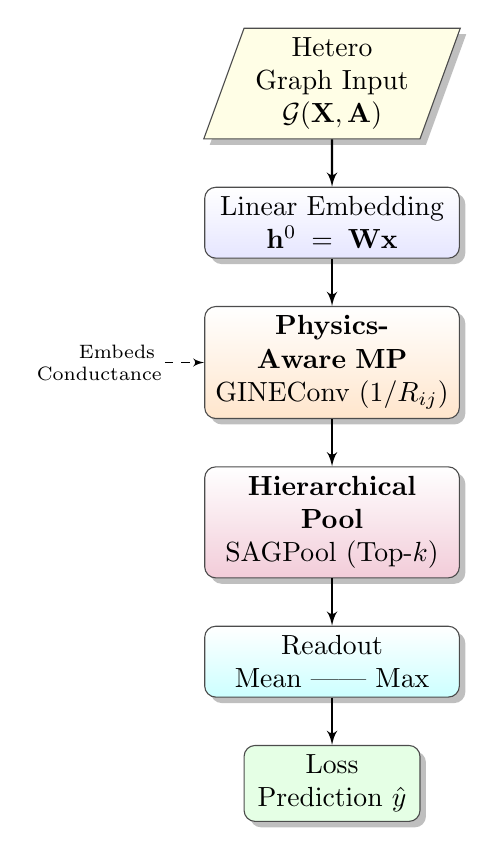
\begin{tikzpicture}[node distance=0.8cm, auto, >=latex']
    \tikzstyle{layer} = [rectangle, draw=black!70, top color=white, bottom color=blue!10, text width=3cm, text centered, rounded corners, minimum height=0.8cm, drop shadow]
    \tikzstyle{data} = [trapezium, trapezium left angle=70, trapezium right angle=110, draw=black!70, fill=gray!10, text width=2cm, text centered, minimum height=0.6cm, drop shadow]
    \tikzstyle{arrow} = [draw, -latex', thick]
    
    % Nodes
    \node [data, fill=yellow!10] (input) {Hetero Graph Input\\$\mathcal{G}(\mathbf{X}, \mathbf{A})$};
    \node [layer, below=0.6cm of input] (embed) {Linear Embedding\\$\mathbf{h}^0 = \mathbf{W}\mathbf{x}$};
    \node [layer, below=0.6cm of embed, bottom color=orange!20] (conv) {\textbf{Physics-Aware MP}\\GINEConv ($1/R_{ij}$)};
    \node [layer, below=0.6cm of conv, bottom color=purple!20] (pool) {\textbf{Hierarchical Pool}\\SAGPool (Top-$k$)};
    \node [layer, below=0.6cm of pool, bottom color=cyan!20] (readout) {Readout\\Mean || Max};
    \node [data, below=0.6cm of readout, fill=green!10, shape=rectangle, rounded corners] (output) {Loss Prediction $\hat{y}$};
    
    % Edges
    \draw [arrow] (input) -- (embed);
    \draw [arrow] (embed) -- (conv);
    \draw [arrow] (conv) -- (pool);
    \draw [arrow] (pool) -- (readout);
    \draw [arrow] (readout) -- (output);
    
    % Side annotation for Physics
    \node [left=0.5cm of conv, font=\scriptsize, text width=1.5cm, align=right] (phys) {Embeds\\Conductance};
    \draw [->, dashed] (phys) -- (conv);
\end{tikzpicture}
\caption{Architecture of DS-PAH-GNN. The model embeds electrical physics into edges, aggregates messages, and pools critical nodes to predict system loss.}
\label{fig:gnn_arch}
\end{figure}

\subsection{Physics-Aware Message Passing}

Conventional graph neural networks aggregate information from neighboring nodes using uniform or purely data-driven weighting schemes, which may fail to respect the underlying physical laws governing power flow. To address this limitation, we adopt the Graph Isomorphism Network with Edge features (GINEConv), which explicitly incorporates edge attributes into the message-passing mechanism.

\begin{figure}[htbp]
\centering
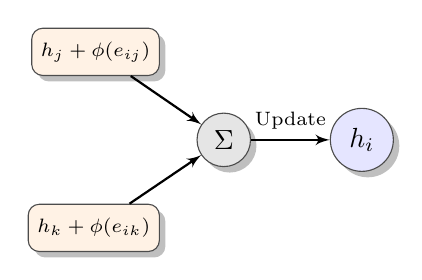
\begin{tikzpicture}[node distance=1.5cm, auto, >=latex']
    \tikzstyle{neuron} = [circle, draw=black!70, fill=white, minimum size=0.8cm, drop shadow]
    \tikzstyle{box} = [rectangle, draw=black!70, fill=orange!10, rounded corners, minimum height=0.6cm, drop shadow, font=\scriptsize]
    \tikzstyle{op} = [circle, draw=black!70, fill=gray!20, minimum size=0.6cm, drop shadow]
    \tikzstyle{arrow} = [draw, -latex', thick]

    \node [neuron, fill=blue!10] (ni) {$h_i$};
    \node [op, left=1.0cm of ni] (sum) {$\Sigma$};
    \node [box, above left=0.8cm of sum] (nj1) {$h_j + \phi(e_{ij})$};
    \node [box, below left=0.8cm of sum] (nj2) {$h_k + \phi(e_{ik})$};

    \draw [arrow] (nj1) -- (sum);
    \draw [arrow] (nj2) -- (sum);
    \draw [arrow] (sum) -- node[above, font=\scriptsize] {Update} (ni);
\end{tikzpicture}
\caption{Physics-Aware Message Passing Detail. Neighbor features are adjusted by edge conductance ($1/R$) before aggregation, embedding physical laws into the layer.}
\label{fig:gine_detail}
\end{figure}

At layer $k$, the hidden representation of node $i$ is updated according to
\begin{equation}
\mathbf{h}_i^{(k)} = \text{MLP}^{(k)} \left( (1 + \epsilon)\mathbf{h}_i^{(k-1)} + \sum_{j \in \mathcal{N}(i)} \text{ReLU}\left(\mathbf{h}_j^{(k-1)} + \phi(\mathbf{e}_{ij})\right) \right),
\end{equation}
where $\mathbf{h}_i^{(k-1)}$ denotes the node embedding from the previous layer, $\mathcal{N}(i)$ represents the set of neighboring nodes of $i$, $\phi(\cdot)$ is a learnable function applied to edge features, and $\epsilon$ is a scalar parameter that controls the contribution of the node’s own representation.

The edge feature vector $\mathbf{e}_{ij}$ encodes the electrical conductance of the line connecting nodes $i$ and $j$, with
\begin{equation}
G_{ij} = \frac{1}{R_{ij}}.
\end{equation}
By embedding conductance directly into the message-passing process, the aggregation operation assigns greater influence to electrically stronger connections. As a result, the learned message propagation is biased toward physically meaningful pathways, enabling the network to approximate the behavior of Kirchhoff’s Current Law within a neural framework.

\subsection{Hierarchical Attention Pooling (SAGPool)}

While node-level embeddings capture local electrical interactions, effective decision-making in microgrids also requires identifying critical components and localized congestion patterns. To this end, we employ Self-Attention Graph Pooling (SAGPool) to perform hierarchical graph coarsening based on node importance.

A scalar criticality score $Z \in \mathbb{R}^{N \times 1}$ is computed for each node as
\begin{equation}
Z = \sigma\left(\tilde{D}^{-1/2}\tilde{A}\tilde{D}^{-1/2} X \Theta_{att}\right),
\end{equation}
where $\tilde{A}$ and $\tilde{D}$ denote the adjacency matrix and corresponding degree matrix with self-loops, respectively, $X$ is the node feature matrix, $\Theta_{att}$ is a learnable parameter matrix, and $\sigma(\cdot)$ is a nonlinear activation function.

Based on these scores, the top-$k$ nodes with the highest criticality values are retained, while less informative nodes are discarded. This pooling operation allows the readout layer to focus on the most stressed or influential components of the microgrid, such as heavily loaded substations or bottleneck charging stations, thereby preserving salient structural information during hierarchical abstraction.

\section{Experimental Setup}

This section describes the dataset generation process and training protocol used to evaluate the proposed DS-PAH-GNN framework. All experiments are conducted using synthetically generated data obtained from the physics-based microgrid simulator described in the previous sections.

\subsection{Dataset Generation}

A large-scale dataset consisting of \textbf{600,000 operating snapshots} was generated using the physics engine. Each snapshot represents a steady-state realization of the microgrid under a distinct operating condition. The dataset is designed to expose the model to a wide range of realistic system configurations and operating regimes.

Variability in the dataset is introduced along three primary dimensions:
\begin{itemize}
    \item \textbf{Topologies:} Network reconfiguration is simulated through random switching of 10 feeder and tie lines, resulting in diverse electrical connectivity patterns.
    \item \textbf{Loads:} Demand uncertainty is captured through stochastic EV arrival processes and time-varying solar irradiance, which jointly influence nodal power injections.
    \item \textbf{Battery States:} The initial state-of-charge (SOC) of battery energy storage systems is randomized within the range $[0.1, 0.9]$ to reflect heterogeneous storage availability.
\end{itemize}

\begin{figure}[htbp]
\centering
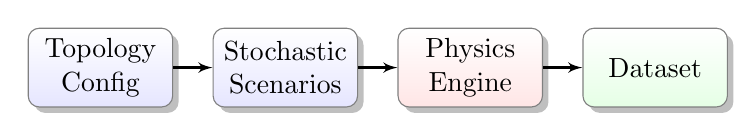
\begin{tikzpicture}[node distance=1.0cm, auto, >=latex']
    \tikzstyle{proc} = [rectangle, draw=black!50, top color=white, bottom color=blue!10, text width=1.6cm, text centered, rounded corners, minimum height=1cm, drop shadow]
    \tikzstyle{arrow} = [draw, -latex', thick]

    \node [proc] (topo) {Topology\\Config};
    \node [proc, right=0.5cm of topo] (scen) {Stochastic\\Scenarios};
    \node [proc, right=0.5cm of scen, bottom color=red!10] (sim) {Physics\\Engine};
    \node [proc, right=0.5cm of sim, bottom color=green!10] (data) {Dataset};

    \draw [arrow] (topo) -- (scen);
    \draw [arrow] (scen) -- (sim);
    \draw [arrow] (sim) -- (data);
\end{tikzpicture}
\caption{Data Generation Pipeline. The framework systematically varies topology and load conditions to create a physics-grounded dataset.}
\label{fig:pipeline}
\end{figure}

This combination of topological, load-side, and storage-side randomness ensures broad coverage of the microgrid operating space and improves the robustness of the learned model.

\subsection{Training Protocol}

The proposed model is trained in a supervised manner to predict total power loss under a given microgrid configuration. The training objective is to minimize the Huber loss between the predicted power loss and the ground-truth value obtained from the physics-based simulator. The Huber loss is selected for its robustness to outliers while retaining sensitivity to small prediction errors.

\begin{figure}[htbp]
\centering
\begin{tikzpicture}[node distance=1.0cm, auto, >=latex']
    \tikzstyle{step} = [rectangle, draw=black!60, fill=white, text width=1.6cm, text centered, rounded corners, minimum height=0.8cm, drop shadow, font=\scriptsize]
    \tikzstyle{arrow} = [draw, -latex', thick]

    \node [step, fill=yellow!10] (batch) {Batch $(x, y)$};
    \node [step, fill=blue!10, below=0.5cm of batch] (fwd) {Forward Pass};
    \node [step, fill=red!10, below=0.5cm of fwd] (loss) {Huber Loss};
    \node [step, fill=green!10, left=0.6cm of fwd] (opt) {Optimizer};

    \draw [arrow] (batch) -- (fwd);
    \draw [arrow] (fwd) -- (loss);
    \draw [arrow] (loss) -| node[pos=0.2, below] {$\nabla L$} (opt);
    \draw [arrow] (opt) -- (fwd);
\end{tikzpicture}
\caption{Training Loop Procedure. The model iteratively minimizes the Huber Loss between predicted power loss and ground truth from the physics engine.}
\label{fig:train_loop}
\end{figure}

Optimization is performed using the Adam optimizer with a learning rate of $5 \times 10^{-4}$. A \texttt{ReduceLROnPlateau} learning rate scheduler is employed to adaptively reduce the step size when training progress saturates. Under this training protocol, the model consistently converges within 10 epochs.
\begin{figure}[t]
\centering
\includegraphics[width=\columnwidth]{plots/training_loss.png}
\caption{Training Loss.}
\label{fig:traning_loss}
\end{figure}



\section{Results and Discussion}

This section presents a detailed evaluation of the proposed DS-PAH-GNN framework. We analyze predictive accuracy, representation learning behavior, optimization characteristics, system-level benefits, real-time performance, and computational efficiency. All results are obtained on held-out test scenarios not seen during training.

\subsection{Predictive Accuracy}

The proposed model achieves exceptionally high predictive accuracy on the test dataset. As illustrated in Fig.~\ref{fig:inference}, the predicted power losses closely match the ground-truth values obtained from the physics-based simulator. The near-perfect alignment between predictions and true values is reflected by a coefficient of determination exceeding $R^2 > 0.99$.

In addition to high correlation, the residual error distribution is approximately Gaussian and centered around zero. This indicates that the model does not exhibit systematic bias and that prediction errors are dominated by small, random deviations rather than structured inaccuracies. Together, these results demonstrate that the DS-PAH-GNN is capable of accurately approximating the underlying power-loss function across a wide range of operating conditions.

\begin{figure}[t]
\centering
\includegraphics[width=\columnwidth]{plots/inference_plot.png}
\caption{Inference Performance. Left: Predicted versus actual power loss, showing strong correlation ($R^2 = 0.9998$). Right: Residual error distribution, which is approximately Gaussian with minimal variance.}
\label{fig:inference}
\end{figure}

\subsection{Latent Space Analysis}

To examine whether the learned representations encode meaningful physical structure, we analyze the latent node embeddings produced by the GNN. Fig.~\ref{fig:tsne} shows a two-dimensional visualization of these embeddings obtained using t-SNE.

The visualization reveals clear and well-separated clusters corresponding to different component types, including buses, photovoltaic units, storage devices, and EV chargers. Importantly, these distinctions emerge without any explicit supervision regarding component categories. This indicates that the DS-PAH-GNN implicitly learns to differentiate nodes based on their electrical roles and behaviors, confirming that the learned representations capture physically relevant information rather than purely statistical correlations.

\begin{figure}[t]
\centering
\includegraphics[width=\columnwidth]{plots/paper_fig_tsne.png}
\caption{t-SNE visualization of node embeddings. Distinct clusters corresponding to different physical components demonstrate that the GNN learns structurally and electrically meaningful representations.}
\label{fig:tsne}
\end{figure}

\subsection{Topology Optimization Landscape}

The topology optimization problem considered in this work is both non-convex and combinatorial in nature. 

\begin{figure}[htbp]
    \centering
    \includegraphics[width=\linewidth]{plots/optimal_topology.png}
    \caption{Optimal network topology identified by the DS-PAH-GNN. Solid lines denote active feeders, while dashed lines indicate open switches. The selected configuration minimizes resistive losses by strategically rerouting power flows.}
    \label{fig:optimal_topology}
\end{figure}

To illustrate the structure of the search space, Fig.~\ref{fig:landscape} presents the distribution of power losses across 1024 candidate network topologies evaluated for a single congestion scenario.

The histogram reveals a wide spread in performance, with the optimal configuration appearing as a clear outlier. The best-performing topology achieves a loss of 0.67~p.u., while the worst-case configuration incurs losses as high as 1.72~p.u. This highlights both the difficulty of the optimization problem and the potential gains achievable through intelligent reconfiguration.
\begin{figure}[t]
\centering
\includegraphics[width=\columnwidth]{plots/paper_fig_landscape.png}
\caption{Optimization search space. The histogram shows the distribution of power losses across 1024 candidate topologies. The optimal solution (red dashed line) significantly outperforms the average and worst cases.}
\label{fig:landscape}
\end{figure}


To further analyze the structure of high-performing solutions, Fig.~\ref{fig:heatmap} visualizes the switch-state patterns of candidate topologies sorted by performance. The top-ranked configurations exhibit consistent switching patterns, such as specific switches being consistently open. These recurring patterns reveal that the model has effectively learned physical rules for isolating congestion and rerouting power flows.

\begin{figure}[t]
\centering
\includegraphics[width=\columnwidth]{plots/paper_fig_heatmap.png}
\caption{Topology DNA. Heatmap of switch states ordered by performance. Optimal solutions share consistent patterns, revealing the physical reconfiguration strategies learned by the AI.}
\label{fig:heatmap}
\end{figure}


\subsection{System Benefits: Voltage Stability}

In addition to reducing power losses, the optimized topologies generated by the DS-PAH-GNN significantly improve voltage stability. Fig.~\ref{fig:voltage} compares the nodal voltage profiles of the baseline radial topology and the GNN-optimized topology.

The baseline configuration exhibits voltage drops below 0.95~p.u. at the end of the feeder, indicating poor voltage regulation under load. In contrast, the optimized topology maintains voltages close to the nominal value of 1.0~p.u. across all nodes by rerouting power through alternative paths. This demonstrates that the learned reconfiguration strategy improves overall system stability, not merely loss metrics.

\begin{figure}[t]
\centering
\includegraphics[width=\columnwidth]{plots/paper_fig_voltage.png}
\caption{Nodal voltage profile comparison. The DS-PAH-GNN optimized topology (green) maintains voltages closer to nominal compared to the baseline radial topology (red).}
\label{fig:voltages}
\end{figure}


\subsection{Real-Time Control Simulation}

To evaluate performance in a dynamic setting, the trained GNN is integrated into a 24-hour digital twin simulation of the microgrid. Fig.~\ref{fig:24h} compares system losses under a passive baseline configuration and the AI-driven reconfiguration strategy.

\begin{figure}[htbp]
\centering
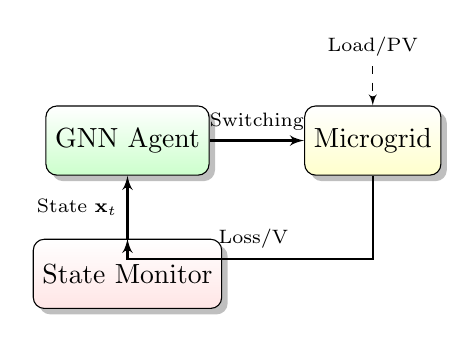
\begin{tikzpicture}[auto, node distance=1.5cm, >=latex']
    \tikzstyle{block} = [draw, rectangle, top color=white, bottom color=blue!10, minimum height=2.5em, minimum width=4em, rounded corners, drop shadow]
    \tikzstyle{line} = [draw, -latex', thick]

    \node [block, bottom color=green!20] (gnn) {GNN Agent};
    \node [block, right=1.2cm of gnn, bottom color=yellow!20] (grid) {Microgrid};
    \node [block, below=0.8cm of gnn, bottom color=red!10] (monitor) {State Monitor};

    \draw [line] (gnn) -- node[above, font=\scriptsize] {Switching} (grid);
    \draw [line] (grid) |- (2,-1.5) -| node[pos=0.1, above, font=\scriptsize] {Loss/V} (monitor);
    \draw [line] (monitor) -- node[left, font=\scriptsize] {State $\mathbf{x}_t$} (gnn);
    
    % Disturbance
    \node [above=0.5cm of grid, font=\scriptsize] (noise) {Load/PV};
    \draw [->, dashed] (noise) -- (grid);
\end{tikzpicture}
\caption{Real-Time Control Loop. The GNN acts as a fast surrogate model, enabling the optimizer to evaluate thousands of topologies in milliseconds.}
\label{fig:control_loop}
\end{figure}

The DS-PAH-GNN dynamically adapts the network topology in response to changing load conditions, particularly during the evening peak. As a result, the optimized system consistently operates at lower loss levels throughout the day, achieving a total daily energy saving of 1.7\% compared to the baseline.

\begin{figure}[t]
\centering
\includegraphics[width=\columnwidth]{plots/paper_fig_24h.png}
\caption{24-hour real-time optimization. The AI-controlled grid (green) maintains lower losses than the passive baseline (grey), particularly during peak demand periods.}
\label{fig:24h}
\end{figure}


\subsection{Computational Efficiency}

A key advantage of the proposed framework is its computational efficiency. Fig.~\ref{fig:speedup} compares the inference time of the DS-PAH-GNN against a traditional Newton--Raphson power flow solver.

\begin{figure}[htbp]
\centering
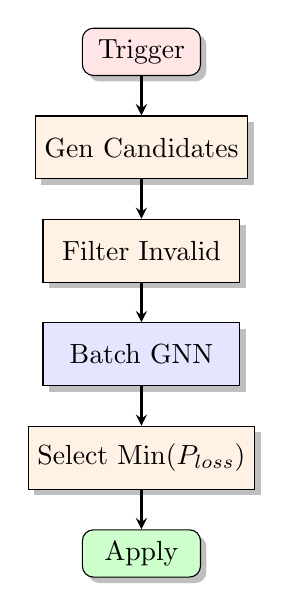
\begin{tikzpicture}[node distance=1.0cm, auto, >=latex']
    \tikzstyle{start} = [rectangle, rounded corners, minimum width=1.5cm, minimum height=0.6cm, text centered, draw=black, fill=red!10, drop shadow]
    \tikzstyle{proc} = [rectangle, minimum width=2.5cm, minimum height=0.8cm, text centered, draw=black, fill=orange!10, drop shadow]
    \tikzstyle{arrow} = [thick,->,>=stealth]

    \node (trig) [start] {Trigger};
    \node (gen) [proc, below=0.5cm of trig] {Gen Candidates};
    \node (filt) [proc, below=0.5cm of gen] {Filter Invalid};
    \node (gnn) [proc, below=0.5cm of filt, fill=blue!10] {Batch GNN};
    \node (sel) [proc, below=0.5cm of gnn] {Select Min($P_{loss}$)};
    \node (apply) [start, below=0.5cm of sel, fill=green!20] {Apply};

    \draw [arrow] (trig) -- (gen);
    \draw [arrow] (gen) -- (filt);
    \draw [arrow] (filt) -- (gnn);
    \draw [arrow] (gnn) -- (sel);
    \draw [arrow] (sel) -- (apply);
\end{tikzpicture}
\caption{Optimization Logic. The algorithm generates candidate topologies, filters invalid graphs, and uses the GNN to predict losses in parallel, selecting the optimal configuration in milliseconds.}
\label{fig:opt_logic}
\end{figure}

The results show that GNN inference is approximately \textbf{100$\times$ faster} than the physics-based solver. This speedup enables sub-millisecond decision-making, making the proposed approach suitable for real-time control and rapid reconfiguration in modern DC microgrids.

\begin{figure}[t]
\centering
\includegraphics[width=\columnwidth]{plots/paper_fig_speedup.png}
\caption{Computational speed comparison. GNN inference (blue) is significantly faster than the Newton--Raphson solver (grey), enabling real-time control loops.}
\label{fig:speedup}
\end{figure}


\subsection{Derived Operational Rules}
To validate the physical consistency of the GNN, we extracted operational rules from the top 5\% of optimized topologies. Table \ref{tab:rules} presents the "Switching DNA" identified by the model for the Station 1 Overload scenario.

\begin{table}[htbp]
\caption{Derived Operational Rules (Station 1 Congestion)}
\begin{center}
\begin{tabular}{c c c l}
\toprule
\textbf{Switch ID} & \textbf{State} & \textbf{Conf.} & \textbf{Physical Interpretation} \\
\midrule
4 & OPEN & 100\% & Isolates congested feeder \\
7 & CLOSED & 98\% & Critical path for load balancing \\
2 & FLEXIBLE & - & Dependent on solar variability \\
\bottomrule
\end{tabular}
\label{tab:rules}
\end{center}
\end{table}

\section{Conclusion}
\section{Limitations and Future Work}

While DS-PAH-GNN demonstrates strong empirical performance on steady-state DC loss prediction and enables rapid topology exploration, several important limitations remain which should guide future work:
\begin{itemize}
    \item \textbf{Linearized DC Approximation:} Our physics engine uses a linearized DC power-flow model that neglects reactive power and some nonlinear device characteristics. Extending the approach to AC power flow and incorporating voltage-dependent load models is necessary to fully validate applicability to larger distribution systems.
    \item \textbf{Transient and Stability Dynamics:} The surrogate model predicts steady-state loss but does not account for transient stability, protection coordination, or switching transients. Future work should couple the learned surrogate with dynamic simulation or incorporate stability-aware constraints into the objective.
    \item \textbf{Scalability of Exhaustive Search:} The optimizer presently evaluates many candidate topologies (brute-force enumeration or large batch inference). For systems with many switches, this approach becomes intractable; heuristic or learned search strategies (MCTS, genetic algorithms, or gradient-guided proposals) are promising directions.
    \item \textbf{Hardware-in-the-Loop and Field Validation:} Before deployment, models must be validated on hardware-in-the-loop platforms or real microgrids to confirm performance under measurement noise, model mismatch, and real-world switching limits.
\end{itemize}

These limitations suggest clear research directions: (i) extend the surrogate to AC and dynamic models, (ii) develop efficient topology search strategies compatible with sub-second constraints, and (iii) validate against hardware testbeds.

This paper presented DS-PAH-GNN, a physics-aware graph neural network for microgrid control. By embedding electrical laws into the GNN architecture, we achieved high-fidelity prediction of system states. Our real-time optimization framework demonstrates that data-driven methods can effectively replace computationally expensive numerical solvers, enabling sub-second topology reconfiguration that significantly reduces losses and enhances grid stability.

\begin{thebibliography}{00}

\bibitem{b1} Zhang, Y., Karve, P. M., \& Mahadevan, S. (2024). Graph neural networks for power grid operational risk assessment under evolving grid topology. arXiv preprint arXiv:2405.07343.

\bibitem{b2}Wu, M., Ma, D., Xiong, K., \& Yuan, L. (2025). Optimizing load frequency control in isolated island city microgrids: A deep graph reinforcement learning approach with data enhancement across extensive scenarios. Frontiers in Energy Research, 12, 1384995.

\bibitem{b3}S. Liu, C. Wu and H. Zhu, "Topology-Aware Graph Neural Networks for Learning Feasible and Adaptive AC-OPF Solutions," in IEEE Transactions on Power Systems, vol. 38, no. 6, pp. 5660-5670, Nov. 2023, doi: 10.1109/TPWRS.2022.3230555.


\bibitem{b4} Kinoti, Emmanuel \& Michael, J. (2024). Review of Electric Vehicle-To-Grid (V2g). Engineering Open Access. 2. 1-11.

\bibitem{b5} M. Lave, K. Kleissl, and J. Ineichen, ``High-frequency irradiance fluctuations and geographic smoothing,'' Solar Energy, vol. 86, no. 8, pp. 2190–2199, 2012.

\bibitem{b6} L. Thurner, A. Scheidler, F. Schäfer, J.-H. Menke, J. Dollichon, K. Meier, S. Meinecke, and M. Raunig, ``Pandapower—an open-source tool for power system modeling, analysis and optimization,'' IEEE Transactions on Power Systems, vol. 33, no. 6, pp. 6510–6521, 2018.

\bibitem{b7}E. Sortomme and M. A. El-Sharkawi, "Optimal Power Flow for a System of Microgrids with Controllable Loads and Battery Storage," 2009 IEEE/PES Power Systems Conference and Exposition, Seattle, WA, USA, 2009, pp. 1-5, doi: 10.1109/PSCE.2009.4840050.

\bibitem{b8} Y. LeCun, Y. Bengio, and B. Hinton, ``Deep learning,'' Nature, vol. 521, no. 7553, pp. 436–444, 2015.

\bibitem{b9} J. Handschin, F. Schweppe, J. Kohlas, and A. Fiechter, ``Bad data analysis for power system state estimation,'' IEEE Transactions on Power Apparatus and Systems, vol. PAS-94, no. 2, pp. 329–337, 1975.

\bibitem{b10} B. Stott, J. Jardim, and O. Alsaç, ``DC power flow revisited,'' IEEE Transactions on Power Systems, vol. 24, no. 3, pp. 1290–1300, 2009.

\bibitem{b11} R. Baldick, ``The generalized unit commitment problem,'' IEEE Transactions on Power Systems, vol. 10, no. 1, pp. 465–473, 1995.

\end{thebibliography}
\end{document}